\documentclass[12pt, letterpaper]{article}
\usepackage{graphicx}
\graphicspath{ {Images/} }

\begin{document}
Assignment 1 Local Search Report

By Brandon Young and Ruicheng Wu

\bigskip

\paragraph{Task 1. Puzzle Representation} \mbox{}\\

\quad GUI Example 1:

\includegraphics[width=\linewidth]{"Task 1/Sample GUI 1"}

\quad GUI Example 2:

\includegraphics[width=\linewidth]{"Task 1/Sample GUI 2"}

\pagebreak

\paragraph{Task 2. Puzzle Evaluation} \mbox{}\\

\quad The puzzle is on the left, while the BFS output is on the right. The following shows 2 puzzles for each possible size, one that is solvable and one that is unsolvable

\medskip
\quad 1. 5x5 (Solvable):
	
\includegraphics[width=3in]{"Task 2/5x5 Puzzle (Solvable)"}

\bigskip
\quad 2. 5x5 (Unsolvable):

\includegraphics[width=3in]{"Task 2/5x5 Puzzle (Unsolvable)"}

\bigskip
\quad 3. 7x7 (Solvable):

\includegraphics[width=4in, keepaspectratio]{"Task 2/7x7 Puzzle (Solvable)"}

\bigskip	
\quad 4. 7x7 (Unsolvable):

\includegraphics[width=4in, keepaspectratio]{"Task 2/7x7 Puzzle (Unsolvable)"}

\bigskip	
\quad 5. 9x9 (Solvable):
	
\includegraphics[width=4in, height=15cm, keepaspectratio]{"Task 2/9x9 Puzzle (Solvable)"}
	
\bigskip
\quad 6. 9x9 (Unsolvable):
	
\includegraphics[width=4in, height=15cm, keepaspectratio]{"Task 2/9x9 Puzzle (Unsolvable)"}


\bigskip
\quad 7. 11x11 (Solvable):
	
\includegraphics[width=5in, keepaspectratio]{"Task 2/11x11 Puzzle (Solvable)"}

\bigskip
\quad 8. 11x11 (Unsolvable):

\includegraphics[width=5in, keepaspectratio]{"Task 2/11x11 Puzzle (Unsolvable)"}

\pagebreak
\paragraph{Task 3. Basic Hill Climb} \mbox{}\\

To get the following plots we ran hill climb 50 times for 3000 iterations and at every 100th iteration we took the K value at that interval. Then we averaged the K values at each interval to get the data for the following scatterplots:

\includegraphics[width=\linewidth]{"Task 3/5x5 Scatterplot"}

\includegraphics[width=\linewidth]{"Task 3/7x7 Scatterplot"}

\includegraphics[width=\linewidth]{"Task 3/9x9 Scatterplot"}

\includegraphics[width=\linewidth]{"Task 3/11x11 Scatterplot"}

\pagebreak
\paragraph{Task 4. Hill Climbing with Random Restarts} \mbox{}\\

For hill climbing with random restarts, using 600 iterations and 5 restarts, the best individual hill climb was picked and its K values were recorded at every 100th iteration:

\includegraphics[width=\linewidth]{"Task 4/5x5 Scatterplot"}

\includegraphics[width=\linewidth]{"Task 4/7x7 Scatterplot"}

\includegraphics[width=\linewidth]{"Task 4/9x9 Scatterplot"}

\includegraphics[width=\linewidth]{"Task 4/11x11 Scatterplot"}

Compared to basic hill climbing, hill climbing with restarts appears to do worse. On the 5x5 plots, for example, restarts only reaches K = 11 at most, but basic hill climb reaches K = 12.

For the number of restarts, more than 2 restarts are preferred, to differentiate from basic hill climb. Yet the number of restarts should not be too high, or the hill climb process will be too short to be effective compared to basic hill climb. So 5 restarts was chosen for the plots above.

\pagebreak
\paragraph{Task 5. Hill Climbing with Random Walking} \mbox{}\\

For hill climbing with random walking, p = 0.01, where p is the probability of allowing downhill movement. A similar process with basic hill climbing was used to obtain the scatterplots below:

\includegraphics[width=\linewidth]{"Task 5/5x5 Scatterplot"}

\includegraphics[width=\linewidth]{"Task 5/7x7 Scatterplot"}

\includegraphics[width=\linewidth]{"Task 5/9x9 Scatterplot"}

\includegraphics[width=\linewidth]{"Task 5/11x11 Scatterplot"}

Random walk does appear to work, however, the dips caused by downhill movement can be too severe to recover from. This is why p was set to 0.01, but it looks like it could be set even lower to retain the effectiveness of basic hill climbing. 

Compared to plain hill climbing and climbing with restarts, random walk performs much worse, reaching a high of about K = 8.5 for 5x5 puzzles while the other 2 methods surpassed 10. However, this may be caused by the averaging of data points, since at some points in the plots, there can be a jump in K values (such as from iterations 800 to 900 on the 9x9 plot).

\pagebreak
\paragraph{Task 6. Simulated Annealing} \mbox{}\\

The parameters used for simulated annealing were: T (initial temperature)= 1000, decay rate = 0.99 with 3000 iterations and every 100th iteration being recorded.

\includegraphics[width=\linewidth]{"Task 6/5x5 Scatterplot"}

\includegraphics[width=\linewidth]{"Task 6/7x7 Scatterplot"}

\includegraphics[width=\linewidth]{"Task 6/9x9 Scatterplot"}

\includegraphics[width=\linewidth]{"Task 6/11x11 Scatterplot"}

Compared to basic hill climbing...

Compared to hill climbing with restarts...

\pagebreak
\paragraph{Task 7. Genetic Algorithms} \mbox{}\\

\begin{document}
	\begin{large}
		In order to run Genetic Algorithm, you need those two sections:\\
		Except Computation Time(It is used by us to record the time before,the feature is unable to use right now), You have a default population size $5$,default mutating probability $0.5$,and default iteration $1$ \\
	\end{large} 
	
	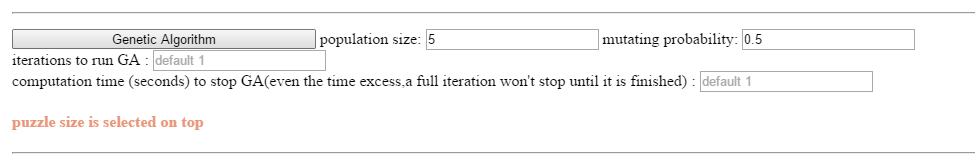
\includegraphics[scale=0.6]{GA-section.png}
	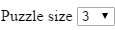
\includegraphics[scale=0.6]{Puzzle-size.png}\\
	
	\begin{large}
		Our implementation of GA is to take a final optimized puzzle(With highest fitness value, K) among all these iterations(default $1$).For each iteration, this method will create puzzle set of population size  $p$ and then evaluate each individual puzzle with fitness function. We select a descent amount of two puzzle groups according to each individuals' fitness value(Some puzzle may not be chosen at all while some may be chosen repeatedly). After selection, we randomly choose one row of puzzles in same group and do this for every group. Then process to cross-over,that is swap Part A of first puzzle with Part A of second puzzle in same group.So now each group should have $PartA-PuzzleOne-PartB-PuzzleTwo$ $PartA-PuzzleTwo-PartB-PuzzleOne$ like structure. The last step is mutating, with corresponding mutating probability,each individual puzzle will have a chance to mutate a randomly selected row(Or may not mutate at all).
	\end{large}
	
	
	(Here, all puzzles are verified and guaranteed to be valid )\\
	
	1,Generating: randomly generate population size $p$ puzzles,store in a Three-Dimensional Array,2D array represents each puzzle.\\
	
	2.Fitness Evaluation and Selection: process each puzzle with fitness function and store corresponding k into an array. Will calculate the total k sum and the proportion of each puzzle, for instance, a k group : $[4,3,2,1]$, the puzzle with ${k=4}$ will be 40 percent and puzzle with $k=1$ will be 10 percent. These probability will be mapping along one line with range $[0,1)$, in this case,$[0,0.4),[0.4,0.7),[0.7,0.9),[0.9,1)$. After storing and mapping k, we use $Math.random()$ to determine the selection. In $Javascript$, $Math.random()$ will generate a number randomly between 0(inclusive),1(exclusive).We check which interval it is located.Do this twice for each selection iteration(an inner loop).According to the combinatorial theory, we decide to run this selection loop until we have either $C(p,2)$ group with no duplicate matrix or this loop has iterated more than population size p(In case the loop stuck when some puzzles with extreme high k being choosing repeatedly or just the order being swapped like $A-B$ and $B-A$).After this loop, we should have a descent amount of group with two puzzles each.\\
	
	(Note : in order to keep a good start, we sort out any puzzle with negative value.)\\
	
	3.Random Pick and Crossing-Over: for each group , use an advanced random number trick to pick a row to cut off and cross over, each group will only need one random number bases their total row numbers. We didn't choose to pick column because it is easier to get entire row than column when we coded(Or if you visualize the $2d$ array as column-row,that is another story).When cross-over, PartA of 1st puzzle will be joined with PartB of 2nd puzzle to make a new puzzle with exact same size as before.And the rest part joined together. Apply this operation to each group, a group of new crossover puzzle is presenting.\\
	
	4.Mutating and Find Best K: Going through all operations before, in our code,randomly pick a row for each puzzle first, then we use random trick again to decide if their chosen rows are going to be mutated or not(We choose to mutate one row instead of one cell).After mutating has done, we present all these puzzles to being evaluated again and capture the puzzle with highest K and draw it and its visualizing matrix on the screen presenting with other data.\\
	
	5.Grand Outer Loop and Harvesting: All operations above are just one run of GA. So we take iteration number to go through GA and harvest the puzzle with highest value K and present it and its visualizing matrix on the screen.\\

\end{document}